\documentclass[a4paper, 12pt]{article}

\usepackage[utf8]{inputenc}
\usepackage[brazilian]{babel}
\usepackage{graphicx}
\usepackage{amssymb, mathrsfs, amsfonts, amsmath, esint, relsize, bm}
\usepackage{hyperref}
\usepackage{caption}
\usepackage{indentfirst} 
\usepackage{xcolor}
\usepackage{csquotes} % When using babel or polyglossia with biblatex, loading csquotes is recommended to ensure that quoted texts are typeset according to the rules of your main language.
\usepackage[ruled,vlined]{algorithm2e} % Algorithm
\usepackage{pdfpages} % Include full PDF file

% References
\usepackage[style=ieee]{biblatex}
\addbibresource{refs.bib}

% \usepackage{hhline}
% \usepackage{color}
% \usepackage{soul}
% \usepackage[table,xcdraw]{xcolor}
% \usepackage{enumerate}

%% My commands
% \newcommand{\myref}[1]{{\color{blue} \ref{#1}}} % Display a blue color for linking figures, tables, equations, etc..
% \newcommand{\mywidth}{.6} % Standard for figures
% \hypersetup{linkcolor=blue, filecolor=magenta, urlcolor=cyan}

% Change background color
% \usepackage{pagecolor,lipsum}% http://ctan.org/pkg/{pagecolor,lipsum}

% \definecolor{maroon}{cmyk}{0,0.87,0.68,0.32}

\begin{document}
% \pagecolor{yellow!50!orange} % ``marcador'' de página feita (movimentas ou comentá-lo de acordo com o avanço do trabalho)

%--------------------------------------------------------------------------
% Capa do relatório
\begin{titlepage}
    \begin{center}
        
\includegraphics[width=2cm]{adj/brasao.png}\\
        {\large {Universidade Federal do Ceará}}\\
        {\large {Centro de Tecnologia}}\\
        {\large {Departamento de Engenharia de Teleinformática}}\\
        {\large {Filtragem Adaptativa - TIP7188}}
    \end{center}

    \vspace{100pt}
    
    \begin{center}
        {\large \textbf {Lista de Exercícios}}
    \end{center}
    
    \vspace{100pt}
    
    \begin{table}[h]
    \begin{tabular}{ll}
        \textbf{Aluno:} Lucas de Souza Abdalah & 539567 \\
    \end{tabular}
    \end{table}
    
    \begin{table}[h]
    \begin{tabular}{l}
        \textbf{Professor:} Charles Casimiro Cavalcante e Guilherme de Alencar Barreto \\
        \textbf{Data de Entrega:} 20/07/2022
    \end{tabular}
    \end{table}
    
    \vspace{\fill}
    
    \begin{center}
        Fortaleza\\
        2022
    \end{center}
    
    \end{titlepage}
    
    %--------------------------------------------------------------------------
    % Sumario do relatorio
    
    \tableofcontents
    \thispagestyle{empty}
    \clearpage

\section{Lista 1: Estatísticas de Segunda Ordem}

\subsection{Média e Autocorrelação}



\subsection{Processos Escationários}

\subsection{Matriz de Autocorrelação}

\subsection{Matriz Definida Positiva}

\subsection{Covariância e correlação}

\subsection{Função de autocorrelação}
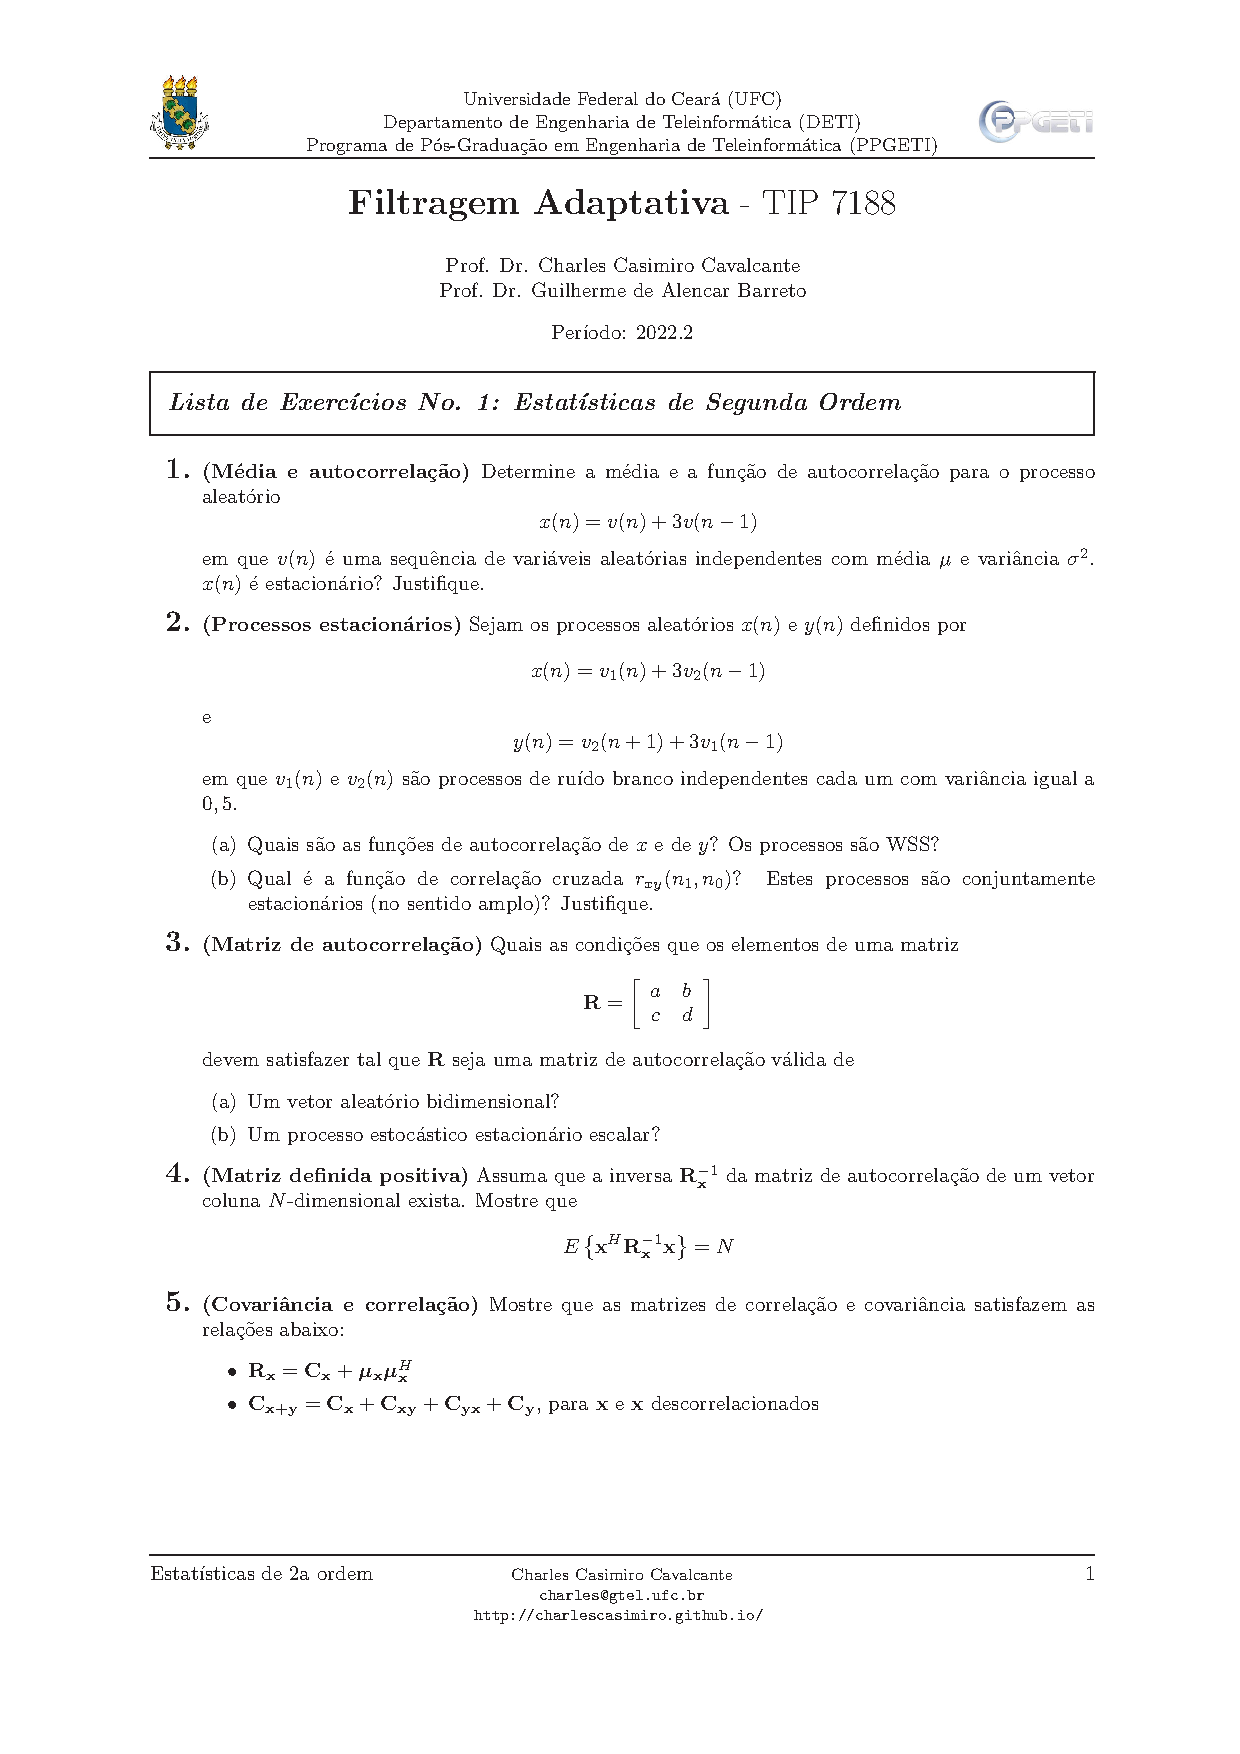
\includepdf[pages={-},addtotoc={1,subsection,1,Exercícios Propostos,p1}]{C:/Users/lucasabdalah-dell/Documents/GitHub/Courses-HWs/Master/TIP7188-FILTRAGEM_ADAPTATIVA/homework/report/listas/Lista_exercicios_1.pdf}
\clearpage
\section{Lista 2: Filtragem Linear Ótima} % <-----------------------------------------------------------------------------


\subsection{Filtragem Ótima} % <-----------------------------------------------------------------------------


\subsubsection*{Coeficientes de Wiener} % <-----------------------------------------------------------------------------

Considerando o problema de filtragem de Wiener, e assumindo conhecimento da matriz de correlação $\mathbf{R_{X}}$ e do vetor de correlação cruzada $\mathbf{p}_{\mathbf{X} d}$, pode-se obter os coeficientes de $\mathbf{w}$.
\begin{equation} 
    \mathbf{w} = \mathbf{R_{X}}^{-1} \mathbf{p}_{\mathbf{X} d} \label{eq:hw2p1}
\end{equation}

Aplicando a equação~\ref{eq:hw2p1}, obtém-se o vetor de pesos do filtro.
\begin{equation*}
    \mathbf{R_{X}}^{-1} =  \left[ \begin{matrix} 1.3333 & -0.6667 \\ -0.6667 & 1.3333 \end{matrix} \right]
\end{equation*}

\begin{align*} 
    \mathbf{w} &= \left[ \begin{matrix} 1.3333 & -0.6667 \\ -0.6667 & 1.3333 \end{matrix} \right] \left[ \begin{matrix} 0.5 \\ 0.25 \end{matrix} \right] \\
        &= \left[ \begin{matrix} 0.5 \\ 0 \end{matrix} \right] \, .
\end{align*}


\subsubsection*{Erro Médio Quadrático}

A partir do vetor de pesos, resultado de~\ref{eq:hw2p1}, basta aplicá-lo na equação do erro mínimo.
\begin{equation}
    \mathbb{E}\{e^{2}(n)\}  =\sigma^{2}_{d} - 2\mathbf{w}^{\top}\mathbf{p}_{\mathbf{X} d} + \mathbf{w}^{\top} \mathbf{R_{X}} \mathbf{w}      
\end{equation}
\begin{align*}
     e &= \sigma^{2}_{d} - 2 \left[ \begin{matrix} 0.5 & 0.0 \end{matrix} \right] \left[ \begin{matrix} 0.5 \\ 0.25 \end{matrix} \right] + \left[ \begin{matrix} 0.5 & 0.0 \end{matrix} \right] \left[ \begin{matrix} 1 & -0.5 \\ -0.5 & 1 \end{matrix} \right]  \left[ \begin{matrix} 0.5  \\ 0.0 \end{matrix} \right] \\
     &= \sigma^{2}_{d} - 2 \times 0.25 + 0.25 \\
     &= \sigma^{2}_{d} - 0.25
\end{align*}


\subsubsection*{Representação em Autovalores}
A decomposição em valores singulares (EVD) pode ser aplicada na matriz de correlação
\begin{equation}
    \mathbf{R}_{X} = \mathbf{Q} \mathbf{\Lambda} \mathbf{Q}^{-1} \label{eq:hw2p1_EVD}
\end{equation}


Aplicando diretamente o resultado da EVD~\ref{eq:hw2p1_EVD} na equação do filtro ótimo~\ref{eq:hw2p1}, obtém-se:
\begin{equation}
    \mathbf{w}= (\mathbf{Q} \mathbf{\Lambda} \mathbf{Q}^{-1})^{-1} \mathbf{p}_{\mathbf{X} d}
\end{equation}

Finalmente, o resultado é uma expressão que compreende a inversão de matrizes menos custosas computacionalmente. Isto se dá principalmente por $\mathbf{\Lambda}$ ser uma matriz diagonal contendo os autovalores da matriz de autocorrelação, bastando calcular $1/\lambda_{i}$ para obter a sua inversa.
\begin{equation}
    \mathbf{w} = \mathbf{Q}^{-1} \mathbf{\Lambda}^{-1} \mathbf{Q} \mathbf{p}_{\mathbf{X} d}.
\end{equation}
                                         

\subsection{Erro Médio Quadrático Mínimo} % <-----------------------------------------------------------------------------
Para verificar a expressão proposta, é necessário obter a matriz de correlação do vetor aumentado.
\begin{align*}
    \mathbf{A} &= \mathbb{E} \left\{ \left[ \begin{matrix} d(n) \\ x(n) \end{matrix} \right] \left[ \begin{matrix} d(n)^{\top} & x(n)^{\top} \end{matrix} \right] \right\} \\
    &= \left[ \begin{matrix} \mathbb{E}\{d(n) d(n)^{\top}\} & \mathbb{E}\{d(n) x(n)^{\top}\} \\ \mathbb{E}\{x(n) d(n)^{\top}\} & \mathbb{E}\{x(n) x(n)^{\top}\} \end{matrix} \right] \\
    &=  \left[ \begin{matrix} \sigma^{2}_{d} & \mathbf{p}_{\mathbf{X} d}^{\top} \\
        \mathbf{p}_{\mathbf{X} d} & \mathbf{R}_{X} \end{matrix} \right]
\end{align*}

É conveniente observar que ao desenvolver a equação, os elementos resultantes da expressão são todo conhecidos. Multiplicando o resultado obtido pelo vetor $\left[\begin{matrix}1 \\ -w \end{matrix} \right]$ à direita e assumindo o modelo nas condições de filtragem ótima, dado filtro de wiener, onde, $\mathbf{w}_{\text{opt}} = \mathbf{R}^{-1}_{X} \mathbf{p}_{\mathbf{X} d}$, temos que:

\begin{align*}
    \mathbf{A} \left[ \begin{matrix} 1 \\ -\mathbf{w} \end{matrix} \right] &= \left[ \begin{matrix} \sigma^{2}_{d} & \mathbf{p}_{\mathbf{X} d}^{\top} \\
        \mathbf{p}_{\mathbf{X} d} & \mathbf{R}_{X} \end{matrix} \right] \left[ \begin{matrix} 1 \\ -\mathbf{w} \end{matrix} \right] \\
        &=   \left[ \begin{matrix} \sigma^{2}_{d} - \mathbf{p}_{\mathbf{X} d}^{\top}\mathbf{w} \\ \mathbf{p}_{\mathbf{X} d} - \mathbf{R}_{X}\mathbf{w} \end{matrix} \right] \\
        &=   \left[ \begin{matrix} \sigma^{2}_{d} - \mathbf{p}_{\mathbf{X} d}^{\top}\mathbf{R}^{-1}_{X} \mathbf{p}_{\mathbf{X} d} \\
            \mathbf{p}_{\mathbf{X} d} - \mathbf{R}_{X}\mathbf{R}^{-1}_{X} \mathbf{p}_{\mathbf{X} d} \end{matrix} \right] \\
        &=   \left[ \begin{matrix} \sigma^{2}_{d} - \mathbf{p}_{\mathbf{X} d}^{\top}\mathbf{R}^{-1}_{X} \mathbf{p}_{\mathbf{X} d} \\
            \mathbf{p}_{\mathbf{X} d} - \mathbf{I}_{X}\mathbf{p}_{\mathbf{X} d} \end{matrix} \right] \\
        &=   \left[ \begin{matrix} \sigma^{2}_{d} - \mathbf{p}_{\mathbf{X} d}^{T
            }\mathbf{R}^{-1}_{X} \mathbf{p}_{\mathbf{X} d} \\ 0 \end{matrix} \right]
\end{align*}

Finalmente, dado a equação obtida, com expressão equivalente à $J_{min}$, pode-se escrever a relação proposta.
\begin{align*}
    \mathbf{A} \left[ \begin{matrix} 1 \\ -\mathbf{w} \end{matrix} \right] = \left[ \begin{matrix} J_{min} \\ 0 \end{matrix} \right]
\end{align*}


\subsection{Cancelamento de Ruído} % <-----------------------------------------------------------------------------
\todo[inline, color=yellow!30]{Organizar}

Inicialmente é necessário calcular a equação de erro do sistema aqui proposto

\begin{align}
    e(n) &= x(n) - \hat{v_{1}} = x(n) - \mathbf{w}^{T}v_{2}(n)
\end{align}

Em seguida faz-necessário calcular a função mean square error(MSE) que é facilmente fornecida pela manipulação algébrica abaixo

\begin{align}
    e^{2}(n) &= [x(n) - \mathbf{w}^{T}v_{2}(n)][x(n) - \mathbf{w}^{T}v_{2}(n)]^{T}, \\
    e^{2}(n) &= x^{2}(n) - 2x(n)\mathbf{w}^{T}v_{2}(n) + \mathbf{w}^{T}v_{2}(n)v_{2}^{T}\mathbf{w}.
\end{align}

Sendo considerado que o filtro apresenta coeficientes constantes é possível aplicar o operador Valor Esperado de forma a obter a seguinte relação

\begin{align}
    \mathbb{E}\{e^{2}(n)\} = \mathbb{E}\{x^{2}(n)\} - 2\mathbf{w}^{T}\mathbb{E}\{x(n) v_{2}(n)\} + \mathbf{w}^{T}\mathbb{E}\{v_{2}(n)v_{2}(n)^{T}\} \mathbf{w},& \\
    \mathbb{E}\{e^{2}(n)\} = \sigma^{2}_{x} - 2\mathbf{w}^{T}\mathbf{p}_{xv_{2}} + \mathbf{w}^{T}\mathbf{R}_{v_{2}} \mathbf{w}.&
\end{align}

Por fim, basta encontrar o $\mathbf{w}$ que minimiza o MSE acima. Para chegar a esse fim, calcula-se o gradiante quanto ao $\mathbf{w}$ igualando-se o resultado da operação a zero

\begin{align}
    \nabla_{\mathbf{w}} \mathbb{E}\{e^{2}(n)\} = - 2\mathbf{p}_{xv_{2}} + 2\mathbf{R}_{v_{2}} \mathbf{w} = 0,& \\
    -\mathbf{p}_{xv_{2}} + \mathbf{R}_{v_{2}} \mathbf{w} = 0,& \\
    \mathbf{R}_{v_{2}} \mathbf{w} = \mathbf{p}_{xv_{2}}.&
\end{align}

Utilizando a identidade matricial abaixo é possível resolver a equação acima para obter o seguinte resultado

\begin{align}
    \mathbf{R}^{-1}_{v_{2}}\mathbf{R}_{v_{2}} \mathbf{w} &= \mathbf{R}^{-1}_{v_{2}}\mathbf{p}_{xv_{2}}, \\
    \mathbf{I}\mathbf{w} &= \mathbf{R}^{-1}_{v_{2}}\mathbf{p}_{xv_{2}}, \\ 
    \mathbf{w} &= \mathbf{R}^{-1}_{v_{2}}\mathbf{p}_{xv_{2}}. 
\end{align}

Onde é possível reescrever o termo final como

\begin{align}
    \mathbf{w} = \mathbf{R}^{-1}_{v_{2}}(\mathbf{p}_{d} + \mathbf{p}_{v_{1}} + \mathbf{p}_{v_{2}}) 
\end{align}


\subsection{Predição Ótima} % <-----------------------------------------------------------------------------
\todo[inline, color=yellow!30]{Organizar}

O filtro linear ótimo que minimiza o erro médio quadrático é descrito pela solução das equações de Wiener. Portanto, inicialmente definir a matriz de autocorrelação para o processo descrito por $x(n)$

\begin{align} 
    \mathbf{R}_{x} = 
    \begin{bmatrix}
        \mathbb{E}\{x(n)x^{*}(n)\} & \mathbb{E}\{x(n-1)x^{*}(n)\} \\
        \mathbb{E}\{x(n)x^{*}(n-1)\}  & \mathbb{E}\{x(n-1)x^{*}(n-1)\} 
    \end{bmatrix},
\end{align}

se considerarmos que o processo $S(n)$ é WSS com variância $\sigma^{2}_{s}$ podemos calcular as correlações como se segue

\begin{align*} 
    \mathbb{E}\{x(n)x^{*}(n)\} &= \mathbb{E}\{ s(n - a) s^{*}(n - a) + s(n - a) s^{*}(n - 4a) + s(n - 4a) s^{*}(n - a) \\
    &+ s(n - 4a) s^{*}(n - 4a) \} = \sigma^{2}_{s} + 0 + 0 + \sigma^{2}_{s} = 2\sigma^{2}_{s} , \\
    \mathbb{E}\{x(n-1)x^{*}(n)\} &= \mathbb{E}\{ s(n - 1 -a) s^{*}(n - a) + s(n - 1 - a) s^{*}(n - 4a) + s(n - 1 - 4a) s^{*}(n - a) \\
    &+ s(n - 1 - 4a) s^{*}(n - 4a) \} = 0 + 0 + 0 + 0 = 0, \\
    \mathbb{E}\{x(n)x^{*}(n-1)\} &= \mathbb{E}\{ s(n - a) s^{*}(n - 1 - a) + s(n - a) s^{*}(n - 1 - 4a) + s(n - 4a) s^{*}(n - 1 - a) \\
    &+ s(n - 4a) s^{*}(n - 1 - 4a) \} = 0 + 0 + 0 + 0 = 0, \\
    \mathbb{E}\{x(n-1)x^{*}(n-1)\} &= \mathbb{E}\{ s(n - 1 -a) s^{*}(n - 1 - a) + s(n - 1 - a) s^{*}(n - 1 - 4a) \\
    &+ s(n - 1 - 4a) s^{*}(n - 1 - a) + s(n - 1 - 4a) s^{*}(n - 1 - 4a) \} = \sigma^{2}_{s} + 0 + 0 + \sigma^{2}_{s} = 2\sigma^{2}_{s}, \\
\end{align*}

obtendo assim

\begin{align} 
    \mathbf{R}_{x} = 
    \begin{bmatrix}
        2 \sigma^{2}_{s} & 0 \\
        0  & 2 \sigma^{2}_{s}
    \end{bmatrix}.
\end{align}

Entretanto, considerando que o processo $D(n)$ têm média nula então temos na verdade um vetor de correlação cruzada nulo. Desse modo, o filtro linear
ótimo para esse processo seria o próprio vetor nulo. Sendo assim

\begin{align} 
    \mathbf{w}_{\text{opt}} = \mathbf{R}^{-1}_{x} \mathbf{p}_{xd} = 
    \begin{bmatrix}
        2 \sigma^{2}_{s} & 0 \\
        0  & 2 \sigma^{2}_{s}
    \end{bmatrix}
    \begin{bmatrix}
        0 \\
        0 
    \end{bmatrix} = 
    \begin{bmatrix}
        0 \\
        0 
    \end{bmatrix},  
\end{align}


\subsection{Superfície de Erro} % <-----------------------------------------------------------------------------
\todo[inline, color=yellow!30]{Organizar}


A partir dos coeficientes fornecidos é possível escrever a matrix de correlação necessário para o filtro ótimo de wiener como uma matriz identidade de ordem 2
						
\begin{align}
    \mathbf{R}_{X} = \left[ \begin{matrix} 1 & 0 \\ 0 & 1 \end{matrix} \right]
\end{align}

Ao utilizar a solução fechada do problema chega-se ao seguinte vetor resultado

\begin{align}
    \mathbf{w}_{\text{opt}} &= \mathbf{R}^{-1}_{x} \mathbf{p}_{xd} = \left[ \begin{matrix} 1 & 0 \\ 0 & 1 \end{matrix} \right]  \left[ \begin{matrix} 2 \\ 4.5 \end{matrix} \right] = \left[ \begin{matrix} 2 \\ 4.5 \end{matrix} \right].
\end{align}

A superfície definida por $J(\mathbf{w})$. Faça um gráfico da mesma.

\textcolor{red}{Solução:}

Para obter a expressão que define a superfície basta desenvolver a expressão para o erro médio

\begin{align}
    \mathbf{J}(w) &= \mathbb{E}\{e^{2}(n)\} = \sigma^{2}_{d} - 2\mathbf{w}^{T}\mathbf{p}_{xd} + w^{T}\mathbf{R}_{X}\mathbf{w}. \label{eq:mse}   
\end{align}

Substituindo os valores encontrados anteriormente na expressão da superfície

\begin{align}
    \mathbf{J}(w_{0}, w_{1}) &= 24.40 - 2 \left[ \begin{matrix} w_{0}  w_{1} \end{matrix} \right] \left[ \begin{matrix} 2 \\ 4.5 \end{matrix} \right] + \left[ \begin{matrix} w_{0}  w_{1} \end{matrix} \right] \left[ \begin{matrix} 1 & 0 \\ 0 & 1 \end{matrix} \right]  \left[ \begin{matrix} w_{0}  \\ w_{1} \end{matrix} \right], \\
    \mathbf{J}(w_{0},w_{1}) &= 24.40 - 4w_{0} - 9w_{1} + w^{2}_{0} + w^{2}_{1}.
\end{align}

Utilizando um software gráfico é possível obter a Figura \ref{fig:hw2p5} onde é traçada a superfície de erro MSE expressa na Equação (\ref{eq:mse}).

\begin{figure}[!htb]
    \centering
    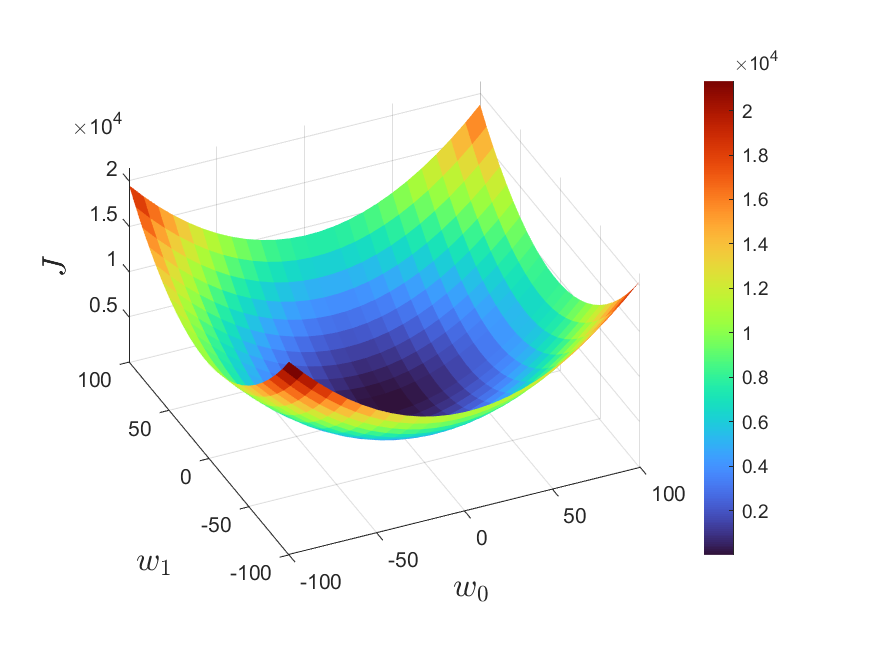
\includegraphics[width=1.0\textwidth]{C:/Users/lucasabdalah-dell/Documents/GitHub/Courses-HWs/Master/TIP7188-FILTRAGEM_ADAPTATIVA/homework/code/figures/hw2p5.pdf}
    \caption{Superfície de erro $J(w_{0}, w_{1})$.}
    \label{fig:hw2p5}
\end{figure}


\clearpage
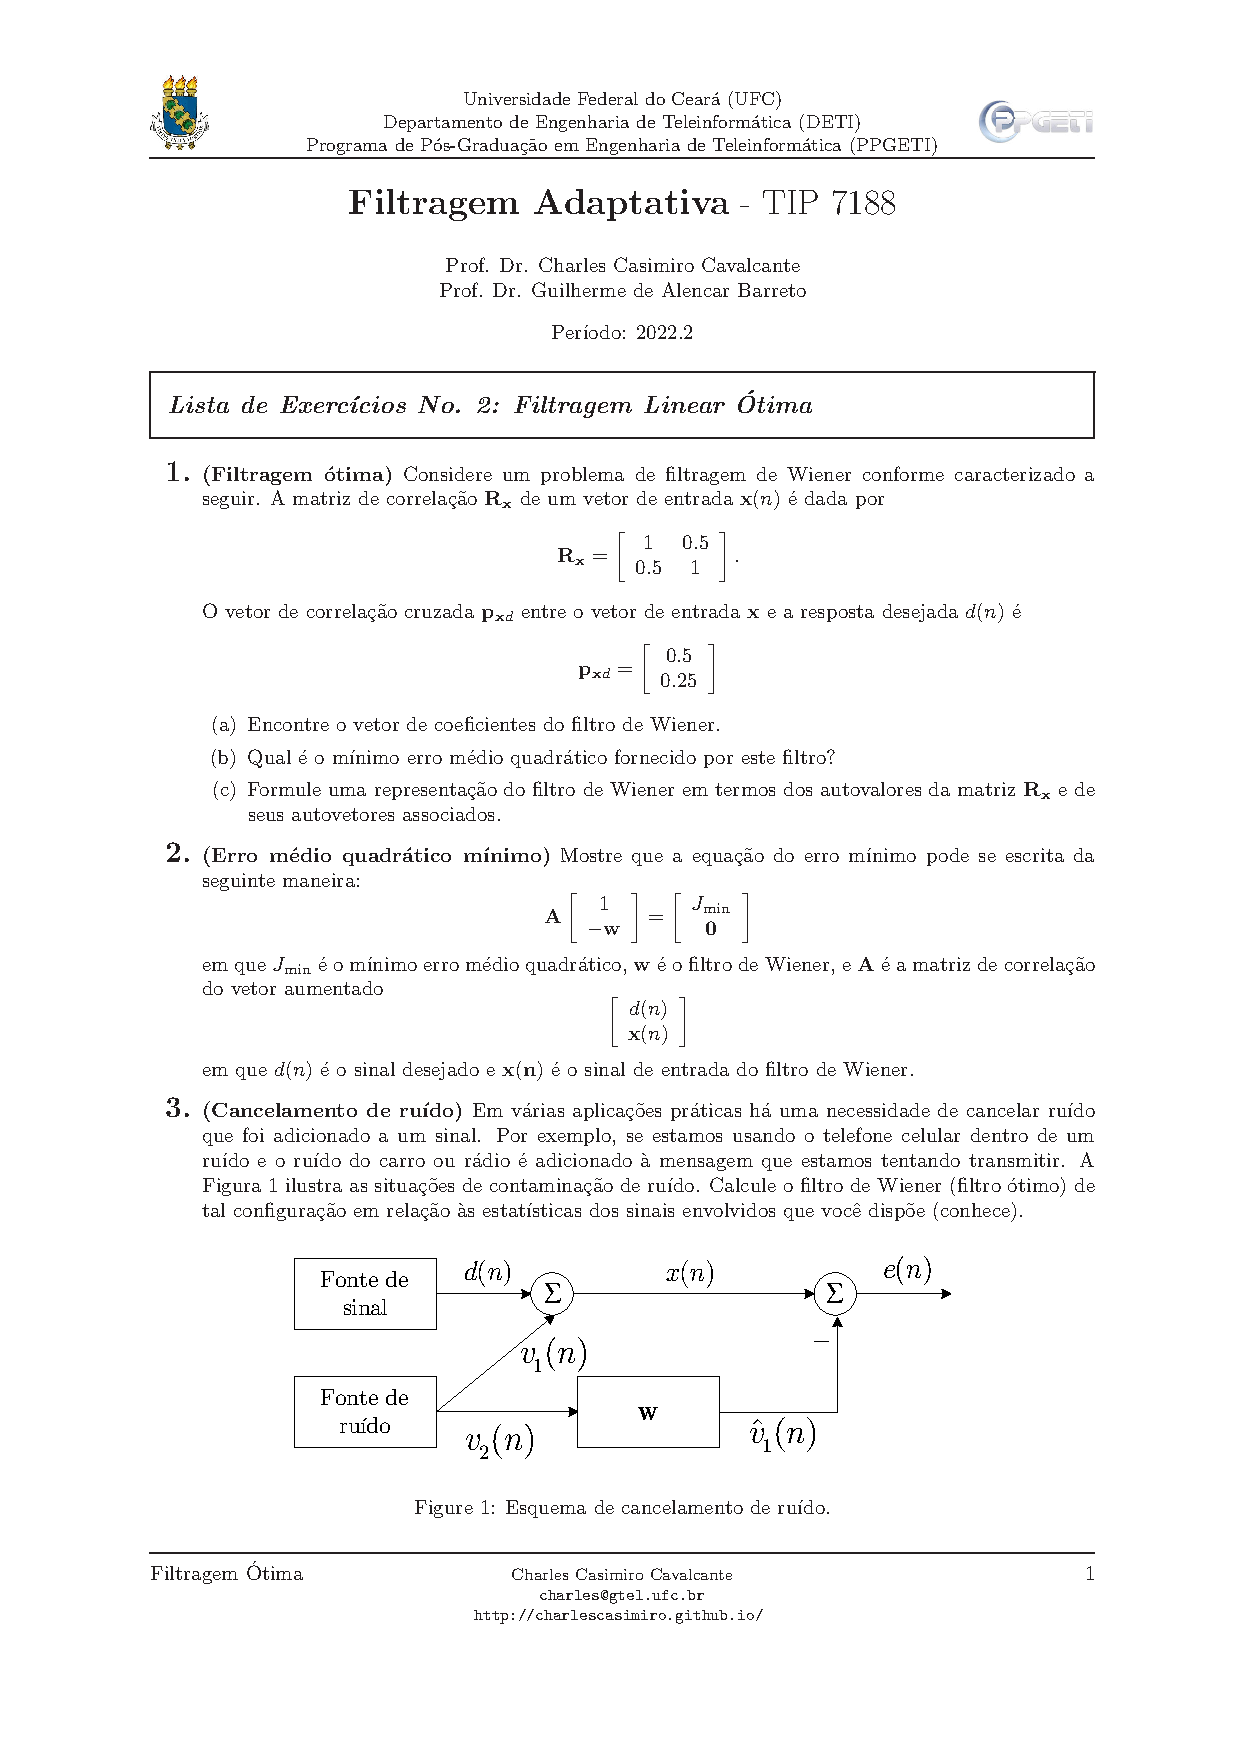
\includepdf[pages={-},addtotoc={1,subsection,1, Exercícios Propostos,p2}]{C:/Users/lucasabdalah-dell/Documents/GitHub/Courses-HWs/Master/TIP7188-FILTRAGEM_ADAPTATIVA/homework/report/listas/Lista_exercicios_2.pdf}
\clearpage
\section{Lista 3: Algoritmos Recursivos}

\subsection{Algoritmo LMF}

\subsection{Algoritmo LMS}

\subsection{Algoritmo LMS Normalizado}

\subsection{Equalização de Canais}

\subsection{Identificação de Sistemas}

\subsection{Equalização Adaptativa}

\clearpage
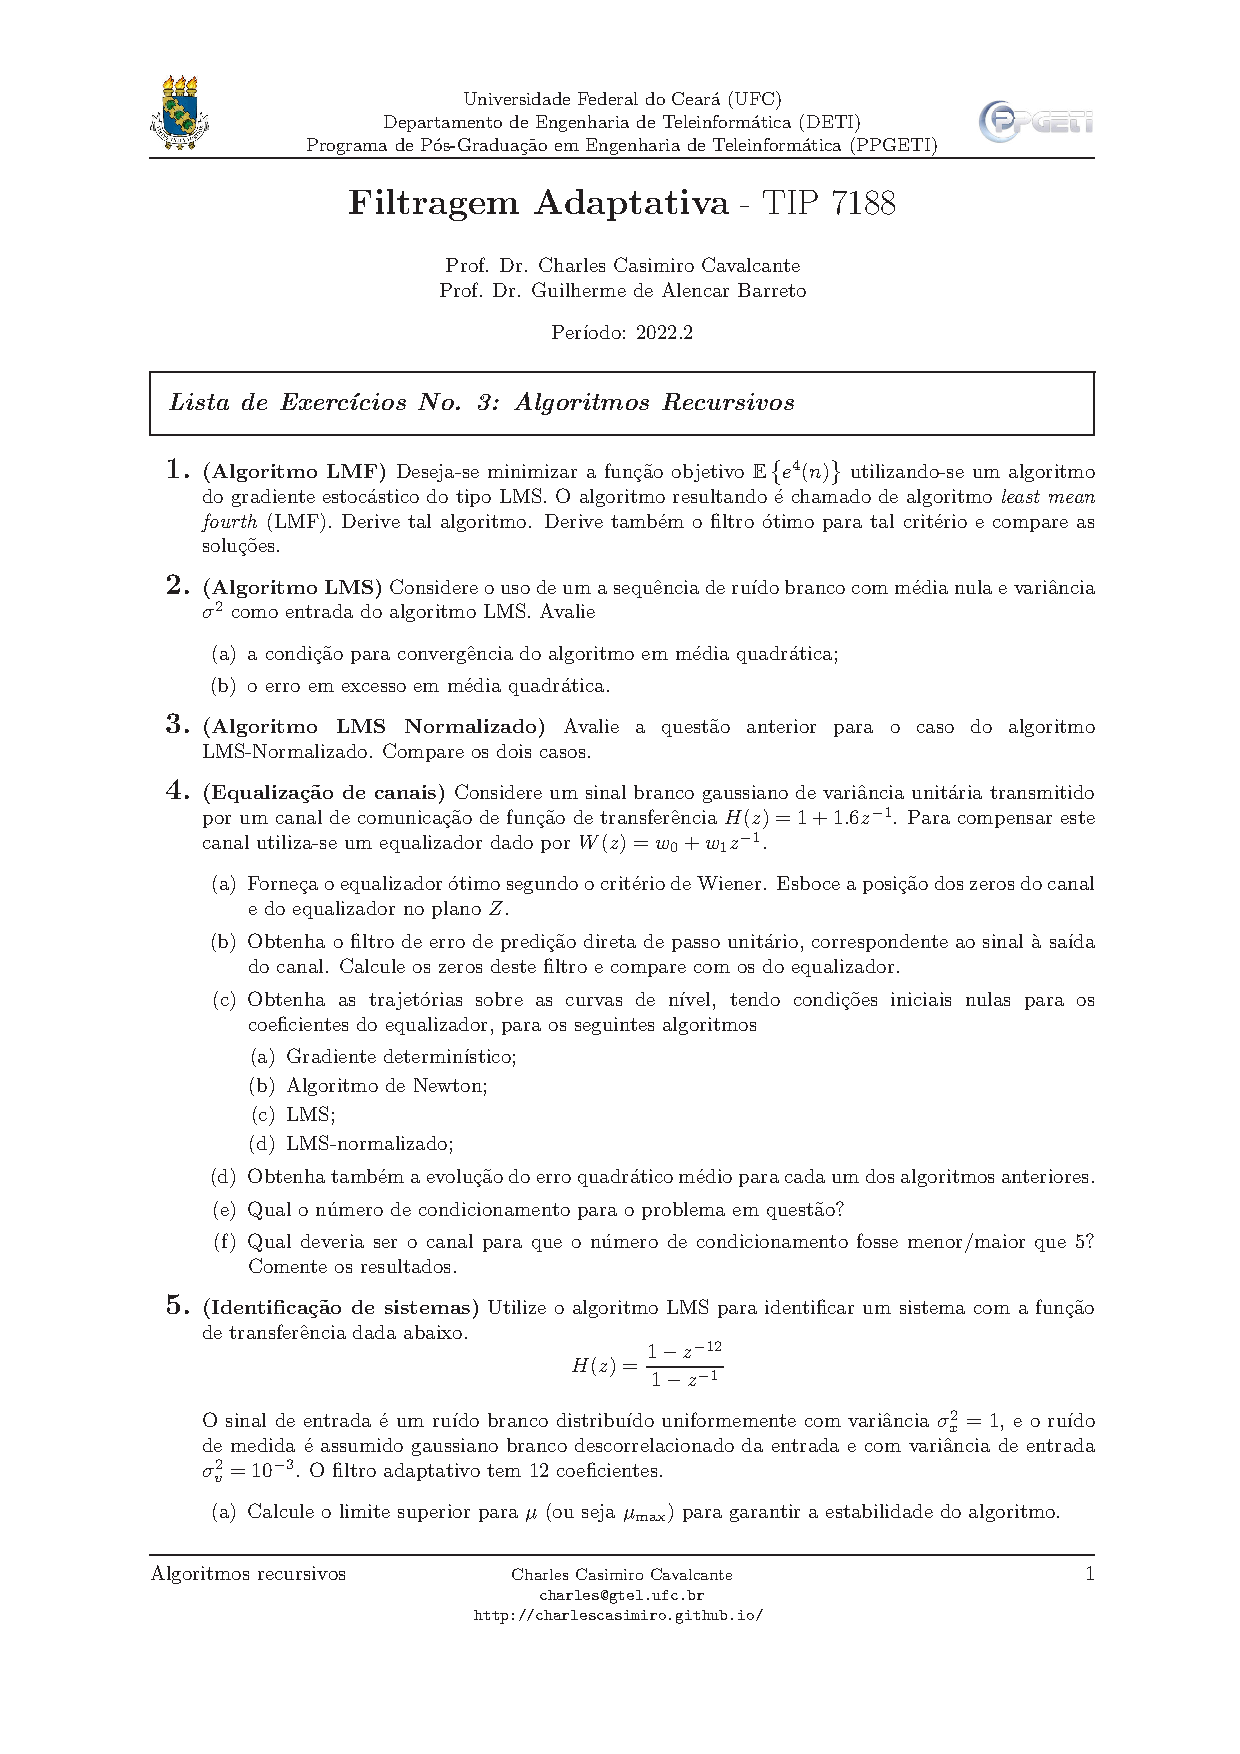
\includepdf[pages={-},addtotoc={1,subsection,1, Exercícios Propostos,p3}]{C:/Users/lucasabdalah-dell/Documents/GitHub/Courses-HWs/Master/TIP7188-FILTRAGEM_ADAPTATIVA/homework/report/listas/Lista_exercicios_3.pdf}
\clearpage
\section{Lista 4: Método dos Mínimos Quadrados} % <-----------------------------------------------------------------------------


\subsection{Algoritmo RLS} % <-----------------------------------------------------------------------------
\todo[inline, color=yellow!30]{Organizar}

\begin{table}[!htp]
    \centering
    \begin{tabular}{|l|l|l|l|}
        \hline
        Iterations & $w_{0}$ & $w_{1}$ & $w_{2}$ \\ 
        \hline 
        i = 1 & 1.0000 & 0.000000 & 0.000000 \\ \hline
        i = 2 & 1.0703 & 0.094579 & 0.087444 \\ \hline
        i = 3 & 0.63832 & 0.67774 & -0.22783 \\ \hline
        i = 4 & 0.25922 & 0.43298 & 0.28991 \\ \hline
        i = 5 & 0.26607 & 0.4316 & 0.28539 \\ \hline
        i = 6 & 0.29342 & 0.40148 & 0.30207 \\ \hline
        i = 7 & 0.29611 & 0.40434 & 0.29579 \\ \hline
        i = 8 & 0.3016 & 0.42552 & 0.27103 \\ \hline
        i = 9 & 0.41718 & 0.35248 & 0.23766 \\ \hline
        i = 10 & 0.38104 & 0.34597 & 0.29742 \\ \hline 
    \end{tabular}
\end{table}

\begin{figure}[!htp]
    \centering
    % \includegraphics[width=0.65\textwidth]{figs/L4Q1.png}
    \includegraphics[width=0.5\textwidth]{example-image}
    \caption{Primeiro coeficiente livre para adaptação com $\text{Amostras} = 100$, $M = 2$, $\lambda = 0.98$}
    \label{fig:L4Q1}
\end{figure}

Na tabela acima foram disponibilizados os coeficientes de filtro para as 10 primeiras iterações como foi pedido. 
A tabela e o algoritmo de filtragem foram implementados utilzando software matemático e os códigos foram disponibilizados junto com 
o relatório. É possível observar nessas primeiras 10 iterações a convergência dos coeficientes de filtro rumo a estabilidade que poderia
ser observada se mais algumas iterações fossem disponibilizadas na tabela. 

Ademais, decidi apresentar o traçado do sinal senoidal transmitido 
comparando-o diretamente com o sinal filtrado na Figura \ref{fig:L4Q1}. É possível conferir que o sinal filtrado começa com uma amplitude bastante
distante do sinal verdadeiro, mas a meddida que mais amostras são utilizadas para a adaptação do sinal a resposta em aplitudade do sinal filtrado se
aproxima do comportamento ideal. Existem algumas oscilações ao longo das 100 amostras, mas sem mudanças abruptas. É necessário apenas chamar atenção 
para o comportamento repentino apresentado no final do processo que é uma consequência da minha implementação para o RLS. Considero que o filtro inicia 
com sua janela totalmente preenchida o que por consequência induz a interupção do algoritmo quando a janela chega a sua última seção onde está totalmente preenchida.

Por fim, na tabela abaixo e na Figura \ref{fig:L4Q2} apresento os resultados para o cenário onde o primeiro coeficiente do filtro RLS é mantido fixo em 1.
Podemos ver de mais imediato que os coeficientes que estão livres para a adaptação apresentam considerável instabilidade quando comparados com o cenário onde os três 
coeficientes estão livres. Consequentemente, o filtro tem uma dificuldade bem maior em acompanhar as mudanças do sinal de referência quando comparamos com o
resultado da Figura \ref{fig:L4Q1}.

\begin{table}[!htp]
    \centering
    \begin{tabular}{|l|l|l|l|}
        \hline
        Iterations & $w_{0}$ & $w_{1}$ & $w_{2}$ \\ 
        \hline 
        i = 1 & 1 & 0 & 0 \\ \hline 
        i = 2 & 1 & -0.043423 & -0.044953 \\ \hline 
        i = 3 & 1 & -0.031108 & -0.038147 \\ \hline 
        i = 4 & 1 & -0.030954 & -0.037966 \\ \hline 
        i = 5 & 1 & -0.021256 & -0.027157 \\ \hline 
        i = 6 & 1 & -0.016635 & -0.01361 \\ \hline 
        i = 7 & 1 & -0.0091408 & -0.0052317 \\ \hline 
        i = 8 & 1 & -0.011328 & -0.0066525 \\ \hline 
        i = 9 & 1 & -0.017649 & -0.00074347 \\ \hline 
        i = 10 & 1 & -0.0095932 & -0.012379 \\ \hline 
    \end{tabular}
\end{table}

\begin{figure}[!htp]
    \centering
    % \includegraphics[width=0.65\textwidth]{figs/L4Q2.png}
    \includegraphics[width=0.5\textwidth]{example-image}
    \caption{Primeiro coeficiente fixo com $\text{Amostras} = 100$, $M = 2$, $\lambda = 0.98$}
    \label{fig:L4Q2}
\end{figure}


\subsection{Erro de Estimação a Priori} % <-----------------------------------------------------------------------------
\todo[inline, color=yellow!30]{Organizar}
    
\begin{align}
    \epsilon(n) = d(n) - \boldsymbol{w}^{\text{H}}(n - 1) \boldsymbol{x}(n),
\end{align}

em que $d(n)$ é a resposta desejada, $x(n)$ é o vetor de entrada do filtro e $\boldsymbol{w}(n - 1)$ é a estimativa
anterior do vetor de coeficientes do filtro. Seja $e(n)$ o erro de estimação a posteriori

\begin{align}
    e(n) = d(n) - \boldsymbol{w}^{\text{H}}(n) \boldsymbol{x}(n),
\end{align}

em que $\boldsymbol{w}(n)$ é a estimativa atual do vetor de coeficientes do filtro. Para dados complexos ambos
$\epsilon(n)$ e $e(n)$ são de valores complexos. Mostre que o produto $\epsilon(n)e^{*}(n)$ é sempre de valor real.

\textcolor{red}{Solução:}

Primeiramente é necessário reescrever $e(n)$ em termos de $\epsilon(n)$. Inicialmente podemos escrever os coeficientes de filtro do instante $n$,
utilizando o erro a priori, da seguinte forma

\begin{align}
    \boldsymbol{w}(n) = \boldsymbol{w}(n-1) + \epsilon(n) \boldsymbol{S}_{D}(n) \boldsymbol{x}(n),
\end{align}

e em seguida substituímos a expressão acima na definição do erro de estimação instantâneo e obtemos 

\begin{align}
    e(n) &= d(n) - \boldsymbol{w}^{\text{H}}(n) \boldsymbol{x}(n), \\
    e(n) &= d(n) - \boldsymbol{x}^{\text{H}}(n) \boldsymbol{w}(n), \\
    e(n) &= d(n) - \boldsymbol{x}^{\text{H}}(n) \left[\boldsymbol{w}(n-1) + \epsilon(n) \boldsymbol{S}_{D}(n) \boldsymbol{x}(n)\right], \\
    e(n) &= d(n) - \boldsymbol{x}^{\text{H}}(n) \boldsymbol{w}(n-1) - \boldsymbol{x}^{\text{H}}(n) \epsilon(n) \boldsymbol{S}_{D}(n) \boldsymbol{x}(n), \\
    e(n) &= \underbrace{d(n) - \boldsymbol{x}^{\text{H}}(n) \boldsymbol{w}(n-1)}_{\epsilon(n)} - \epsilon(n) \boldsymbol{x}^{\text{H}}(n) \boldsymbol{S}_{D}(n) \boldsymbol{x}(n), \\
    e(n) &= \epsilon(n) - \epsilon(n) \boldsymbol{x}^{\text{H}}(n) \boldsymbol{S}_{D}(n) \boldsymbol{x}(n), \\
\end{align}

e em sequência desenvolvemos o conjugado de $e(n)$ do seguinte modo

\begin{align}
    e^{*}(n) &= \epsilon^{*}(n) - \epsilon^{*}(n) \boldsymbol{x}^{\text{H}}(n) \boldsymbol{S}_{D}(n) \boldsymbol{x}(n),
\end{align}

onde o termo $\boldsymbol{x}^{\text{H}}(n) \boldsymbol{S}_{D}(n) \boldsymbol{x}(n)$ é a distância de Mahalanobis que será sempre real e positiva.
Desse modo, ao fazermos $\epsilon(n) e^{*}(n)$ obtemos 

\begin{align}
    \epsilon(n) e^{*}(n) &= \epsilon(n) \left[\epsilon^{*}(n) - \epsilon^{*}(n) \boldsymbol{x}^{\text{H}}(n) \boldsymbol{S}_{D}(n) \boldsymbol{x}(n)\right], \\
    \epsilon(n) e^{*}(n) &= \epsilon(n) \epsilon^{*}(n) - \epsilon(n) \epsilon^{*}(n) \boldsymbol{x}^{\text{H}}(n) \boldsymbol{S}_{D}(n) \boldsymbol{x}(n), \\
    \epsilon(n) e^{*}(n) &= \epsilon(n) \epsilon^{*}(n) \left(1 - \boldsymbol{x}^{\text{H}}(n) \boldsymbol{S}_{D}(n) \boldsymbol{x}(n)\right).
\end{align}

Dessa forma, sabemos que o termos $\left(1 - \boldsymbol{x}^{\text{H}}(n) \boldsymbol{S}_{D}(n) \boldsymbol{x}(n)\right)$ será sempre real, embora nem sempre positivo,
e $\epsilon(n) \epsilon^{*}(n)$ pode simplesmente ser visto como uma norma dada por $||\epsilon(n)||^{2} = \epsilon(n) \epsilon^{*}(n)$, demonstrando assim que sempre 
teremos um valor real para $\epsilon(n) e^{*}(n)$.


\subsection{Preditor Adaptativo} % <-----------------------------------------------------------------------------
\todo[inline, color=yellow!30]{Organizar}
Os resultados podem ser encontrados nas Figuras \ref{fig:L4Q3_a1} - \ref{fig:L4Q3_a8}. Nas figuras \ref{fig:L4Q3_a1} e \ref{fig:L4Q3_a2} temos a evolução
dos coeficientes de filtro e do MSE para o RLS com fator de esquecimento $\lambda = 0.9$, SNR = $3$ dB e ordens $M = 2$ e $M = 3$, respectivamente. Nesses cenários podemos 
ver que o RLS não atingiu a estabilidade em seus coeficientes de filtro embora tenha apresentado um comportamento MSE sem grandes variâncões de magnitude. Ademais, no segundo cenário
é possível verificar maior estabilidade na evolução do MSE graças ao incremento na ordem do RLS. Em sequência, nas Figuras \ref{fig:L4Q3_a3} e \ref{fig:L4Q3_a4} temos dois cenárioss similares, 
mas agora com um fator dde conhecimento igual a $\lambda = 0.99$. Diferentemente dos dois primeiros cenários agora é possível verificar que o RLS atingiu estabilidade em seus coeficientes de filtro, 
além de um melhor desempenho na evolução do MSE do que nos casos anteriores. Isso se deve pois, diferente do que ocorre com o passo de aprendizado nos algoritmos estudados anteriormente, a medida que
$\lambda$ cresce menos fléxivel torna-se o filtro. Desse modo, é mais fácil para esses novos cenários adaptem-se à evolução do canal com maior facilidade. Alem disso, novamente foi possível observar 
o impacto da ordem do RLS na estabilidade da evolução do MSE, onde para o cenário $M = 3$ foi verificado um melhor desempenho do que para o cenário $M = 2$.

Por fim, nos resta analisar o impacto da SNR na estabilidade e desempenho do RLS. Nas Figuras \ref{fig:L4Q3_a5} e \ref{fig:L4Q3_a6} temos o equivalente ao primeiro par de cenários, mas agora 
com a diferença de que ambos os cenários são de SNR infinita. Para o primeiro caso com $M = 2$ vemos uma estabilização perfeita dos coeficientes do filtro e uma evolução do erro MSE que tende ao erro de
precisão da máquina. Dessa forma, podemos considerar esse um cenário ideal para o RLS. Sequencialmente, na figura seguinte consideramos um cenário $M = 3$ e podemos verificar que não existiu convergência para
esse cenário. Inicialmente existiu uma certa estabilização na evolução do MSE, mas apos algumas iterações o filtro perdeu a estabilidade e seus coeficientes "explodiram". Esse comportamento pode ser explicado 
tanto pelo aumento da ordem do filtro quanto pelo fator de esquecimento que torna o filtro muito pouco fléxivel e suscetível a instabilidades provocadas por mudanças repentinas. Por fim, nas Figuras \ref{fig:L4Q3_a7}
e \ref{fig:L4Q3_a8} temos dois resultados estáveis na evolução do MSE e nos coeficientes do filtro RLS. Isso se deve principalmente a um fator de esquecimento que fornece maior capacidade de resistir a instabilidades
geradas pelo canal.

\begin{figure}[!htp]
    \centering
    %\includegraphics[width=0.825\textwidth]{figs/L4Q3_rls_mse_2_3_9.png}
    \includegraphics[width=0.5\textwidth]{example-image}
    \caption{SNR = 3 dB, M = 2 and $\lambda = 0.9$}
    \label{fig:L4Q3_a1}
\end{figure}

\begin{figure}[!htp]
    \centering
    %\includegraphics[width=0.825\textwidth]{figs/L4Q3_rls_mse_3_3_9.png}
    \includegraphics[width=0.5\textwidth]{example-image}
    \caption{SNR = 3 dB, M = 3 and $\lambda = 0.9$}
    \label{fig:L4Q3_a2}
\end{figure}

\begin{figure}[!htp]
    \centering
    %\includegraphics[width=0.825\textwidth]{figs/L4Q3_rls_mse_2_3_99.png}
    \includegraphics[width=0.5\textwidth]{example-image}
    \caption{SNR = 3 dB, M = 2 and $\lambda = 0.99$}
    \label{fig:L4Q3_a3}
\end{figure}

\begin{figure}[!htp]
    \centering
    %\includegraphics[width=0.825\textwidth]{figs/L4Q3_rls_mse_3_3_99.png}
    \includegraphics[width=0.5\textwidth]{example-image}
    \caption{SNR = 3 dB, M = 3 and $\lambda = 0.99$}
    \label{fig:L4Q3_a4}
\end{figure}

\begin{figure}[!htp]
    \centering
    %\includegraphics[width=0.825\textwidth]{figs/L4Q3_rls_mse_2_inf_9.png}
    \includegraphics[width=0.5\textwidth]{example-image}
    \caption{SNR = $\infty$ dB, M = 2 and $\lambda = 0.9$}
    \label{fig:L4Q3_a5}
\end{figure}

\begin{figure}[!htp]
    \centering
    %\includegraphics[width=0.825\textwidth]{figs/L4Q3_rls_mse_3_inf_9.png}
    \includegraphics[width=0.5\textwidth]{example-image}
    \caption{SNR = $\infty$ dB, M = 3 and $\lambda = 0.9$}
    \label{fig:L4Q3_a6}
\end{figure}

\begin{figure}[!htp]
    \centering
    %\includegraphics[width=0.825\textwidth]{figs/L4Q3_rls_mse_2_inf_99.png}
    \includegraphics[width=0.5\textwidth]{example-image}
    \caption{SNR = $\infty$ dB, M = 2 and $\lambda = 0.99$}
    \label{fig:L4Q3_a7}
\end{figure}

\begin{figure}[!htp]
    \centering
    % \includegraphics[width=0.825\textwidth]{figs/L4Q3_rls_mse_3_inf_99.png}
    \includegraphics[width=0.5\textwidth]{example-image}
    \caption{SNR = $\infty$ dB, M = 3 and $\lambda = 0.99$}
    \label{fig:L4Q3_a8}
\end{figure}
\clearpage


\subsection{Equalização de Canais} % <-----------------------------------------------------------------------------
\todo[inline, color=yellow!30]{Organizar}
\begin{enumerate}
    
    \item Calcule a adaptação do algoritmo usando o RLS e mostre a evolução temporal dos coeficientes.

        \textcolor{red}{Solução:}

        A evolução temporal dos coeficientes do filtro pode ser encontrada na Figura \ref{fig:rls_coefficient}.  
        Aqui é possível verificar a convergência e estabilização dos coeficientes do filtro partindo do zero a medida que o número 
        de iterações cresce. Existem algumas oscilações ao final do processo, mas nada considerável. Caso o fator de esquecimento fosse
        aumentado possivelmente haveriam oscilações com maiores magnitudes nos coeficientes de filtro. 

    \item Obtenha as trajetórias sobre as curvas de nível, tendo condições iniciais nulas para os
    coeficientes do equalizador. Verifique qual a melhor inicialização do algoritmo RLS. Compare
    com os algoritmos LMS, LMS-Normalizado e Gauss-Newton.

        \textcolor{red}{Solução:}

        As trajetórias dos algoritmos Newton, Gradiente, LMS e NLMS estão disponíveis nas Figuras \ref{fig:newton_contour}, \ref{fig:gradient_contour}, 
        \ref{fig:lms_contour} e \ref{fig:nlms_contour}. Na Figura \ref{fig:rls_contour} é apresentado o traçado da trajetória de convergência para o RLS.
        É possível verificar que o RLS apresenta um comportamento de convergência na superfície MSE mais próximo do algoritmo LMS. Existem alguns outliers durante 
        o processo de filtragem, mas de modo geral o filtro tende à solução ótima de uma forma mais organizada e estável do que o NLMS.

    \item Obtenha também a evolução do erro quadrático médio para cada um dos algoritmos anteriores.

        \textcolor{red}{Solução:} 

        As evolução do erro quadrático médio para os algoritmos Newton, Gradiente, LMS e NLMS já foram abordadas na seção 
        anterior e podem ser revisitadas nas Figuras \ref{fig:newton_mse}, \ref{fig:gradient_mse}, \ref{fig:lms_mse} e \ref{fig:nlms_mse}.
        adicionalmente, o traçado da evolução do MSE para o método RLS está presente na Figura \ref{fig:rls_mse}. Nessa figura podemos verificar
        que o RLS apresenta uma latência de convergência menor que o LMS e NLMS, mas ao final do processo aparentemente o grau de estabilidade da
        solução dos coeficientes de filtro parece ser menor do que quando comparamos com os quatro algoritmos de filtragem mencionados anteriormente.


\begin{figure}[!htp]
    \centering
    % \includegraphics[width=0.75\textwidth]{figs/rls_coefficients.png}
    \includegraphics[width=0.5\textwidth]{example-image}
    \caption{Convergência dos coeficientes para o RLS. $\text{Amostras} = 5000$, $M = 2$, $\lambda = 0.99$}
    \label{fig:rls_coefficient}
\end{figure}

\begin{figure}[!htp]
    \centering
    % \includegraphics[width=0.75\textwidth]{figs/rls_contour.png}
    \includegraphics[width=0.5\textwidth]{example-image}
    \caption{Caminho de convergência na superficie MSE para o RLS. $\text{Amostras} = 5000$, $M = 2$, $\lambda = 0.99$}
    \label{fig:rls_contour}
\end{figure}

\begin{figure}[!htp]
    \centering
    % \includegraphics[width=0.75\textwidth]{figs/rls_mse.png}
    \includegraphics[width=0.5\textwidth]{example-image}
    \caption{Comportamento da evolução do MSE para o RLS. $\text{Amostras} = 5000$, $M = 2$, $\lambda = 0.99$}
    \label{fig:rls_mse}
\end{figure}

\end{enumerate}


\subsection{Equalização Adaptativa} % <-----------------------------------------------------------------------------
\todo[inline, color=yellow!30]{Organizar}

Assim como na questão da lista anterior foi considerado novamente que o filtro é de ordem $M = 15$.
Os resultados podem ser encontrados nas Figuras \ref{fig:L4Q5_a1}, \ref{fig:L4Q5_a2}, \ref{fig:L4Q5_a3} e \ref{fig:L4Q5_a4}.
Inicialmente é possível confirmar uma evidente vantagem na velocidade de convergência do RLS quando o comparamos com o algoritmo LMS.
Independentemente do fator de esquecimento considerado todos apresentam uma vantagem considerável sobre o LMS quando se observa tanto a 
latência quanto o desempenho da evolução do MSE. Desse modo, o RLS tem menor latência e melhor desempenho MSE quando comparamos com o LMS.

Já quando voltamos nossa análise para o impacto do fator de esquecimento é possível verificar uma interessante característica do 
RLS. O fator de esquecimento atua de forma semelhante ao passo de aprendizado nos algoritmos LMS e NLMS, mas num sentido um  pouco diferente. Desse modo, quanto
maior o seu valor mais flexível torna-se o filtro para adaptar-se a novos estímulos. Assim, nas Figuras \ref{fig:L4Q5_a2} e \ref{fig:L4Q5_a3}, onde o 
fator de esquecimento é definido respectivamente por $\lambda = 0.9$ e $\lambda = 0.99$, é possível ver que o MSE apresenta oscilações de 
elevadas magnitudades mesmo após a convergência pois estamos restringindo a flexibilidade do RLS. Já na Figura \ref{fig:L4Q5_a4} onde temos um fator de esquecimento 
definido por $\lambda = 0.999$ temos oscilações de magnitudades consideravelmente menores quando comparamos com os dois casos anteriores. Já com relação ao valor de convergência
MSE não é possível notar grandes diferenças entre os casos considerados, visto que todos oscilam em torno de um valor aproximadamente igual.

Por fim, nas Figuras \ref{fig:L4Q5_a5} e \ref{fig:L4Q5_a6} são traçados os gráficos da evolução temporal e da resposta em frequência para
o cenário proposto, respectivamente. Na primeira figura vemos a adaptação do algoritmo RLS a medida que o número de iterações progride e, apesar do
equalizador desconhecer o sinal verdadeiro, existe uma aparente melhora de desempenho a medida que o filtro progride. Já na figura seguinte são comparados
diretamente as repostas em frequência dos filtros LMS e RLS em relação ao sistema desconhecido com $\mu = 0.001$ e $\lambda = 0.999$, respectivamente.
A partir de tal resultado podemos verificar que o filtro RLS consegue adaptar-se mais facilmente ao sistema desconhecido enquanto o filtro LMS apresenta
intensas variações que possivelmente prejudicariam o processo de filtragem.


\begin{figure}[!htp]
    \centering
    % \includegraphics[width=0.75\textwidth]{figs/L4Q5_lms.png}
    \includegraphics[width=0.5\textwidth]{example-image}
    \caption{Comportamento da evolução do MSE para o LMS. $\text{Amostras} = 500$, $M = 15$, $\mu = 0.001$}
    \label{fig:L4Q5_a1}
\end{figure}

\begin{figure}[!htp]
    \centering
    % \includegraphics[width=0.75\textwidth]{figs/L4Q5_rls_9.png}
    \includegraphics[width=0.5\textwidth]{example-image}
    \caption{Comportamento da evolução do MSE para o RLS. $\text{Amostras} = 500$, $M = 15$, $\lambda = 0.9$}
    \label{fig:L4Q5_a2}
\end{figure}

\begin{figure}[!htp]
    \centering
    % \includegraphics[width=0.75\textwidth]{figs/L4Q5_rls_99.png}
    \includegraphics[width=0.5\textwidth]{example-image}
    \caption{Comportamento da evolução do MSE para o RLS. $\text{Amostras} = 500$, $M = 15$, $\lambda = 0.99$}
    \label{fig:L4Q5_a3}
\end{figure}

\begin{figure}[!htp]
    \centering
    % \includegraphics[width=0.75\textwidth]{figs/L4Q5_rls_999.png}
    \includegraphics[width=0.5\textwidth]{example-image}
    \caption{Comportamento da evolução do MSE para o RLS. $\text{Amostras} = 500$, $M = 15$, $\lambda = 0.999$}
    \label{fig:L4Q5_a4}
\end{figure}

\begin{figure}[!htp]
    \centering
    % \includegraphics[width=0.75\textwidth]{figs/L4Q5_rls_t.png}
    \includegraphics[width=0.5\textwidth]{example-image}
    \caption{Evolução temporal para o RLS. $\text{Amostras} = 500$, $M = 15$, $\lambda = 0.999$}
    \label{fig:L4Q5_a5}
\end{figure}

\begin{figure}[!htp]
    \centering
    % \includegraphics[width=0.75\textwidth]{figs/L4Q5_filter_response.png}
    \includegraphics[width=0.5\textwidth]{example-image}
    \caption{Comparativo da resposta em frequência para LMS e RLS. $\text{Amostras} = 500$, $M = 15$, $\lambda = 0.999$}
    \label{fig:L4Q5_a6}
\end{figure}


\clearpage
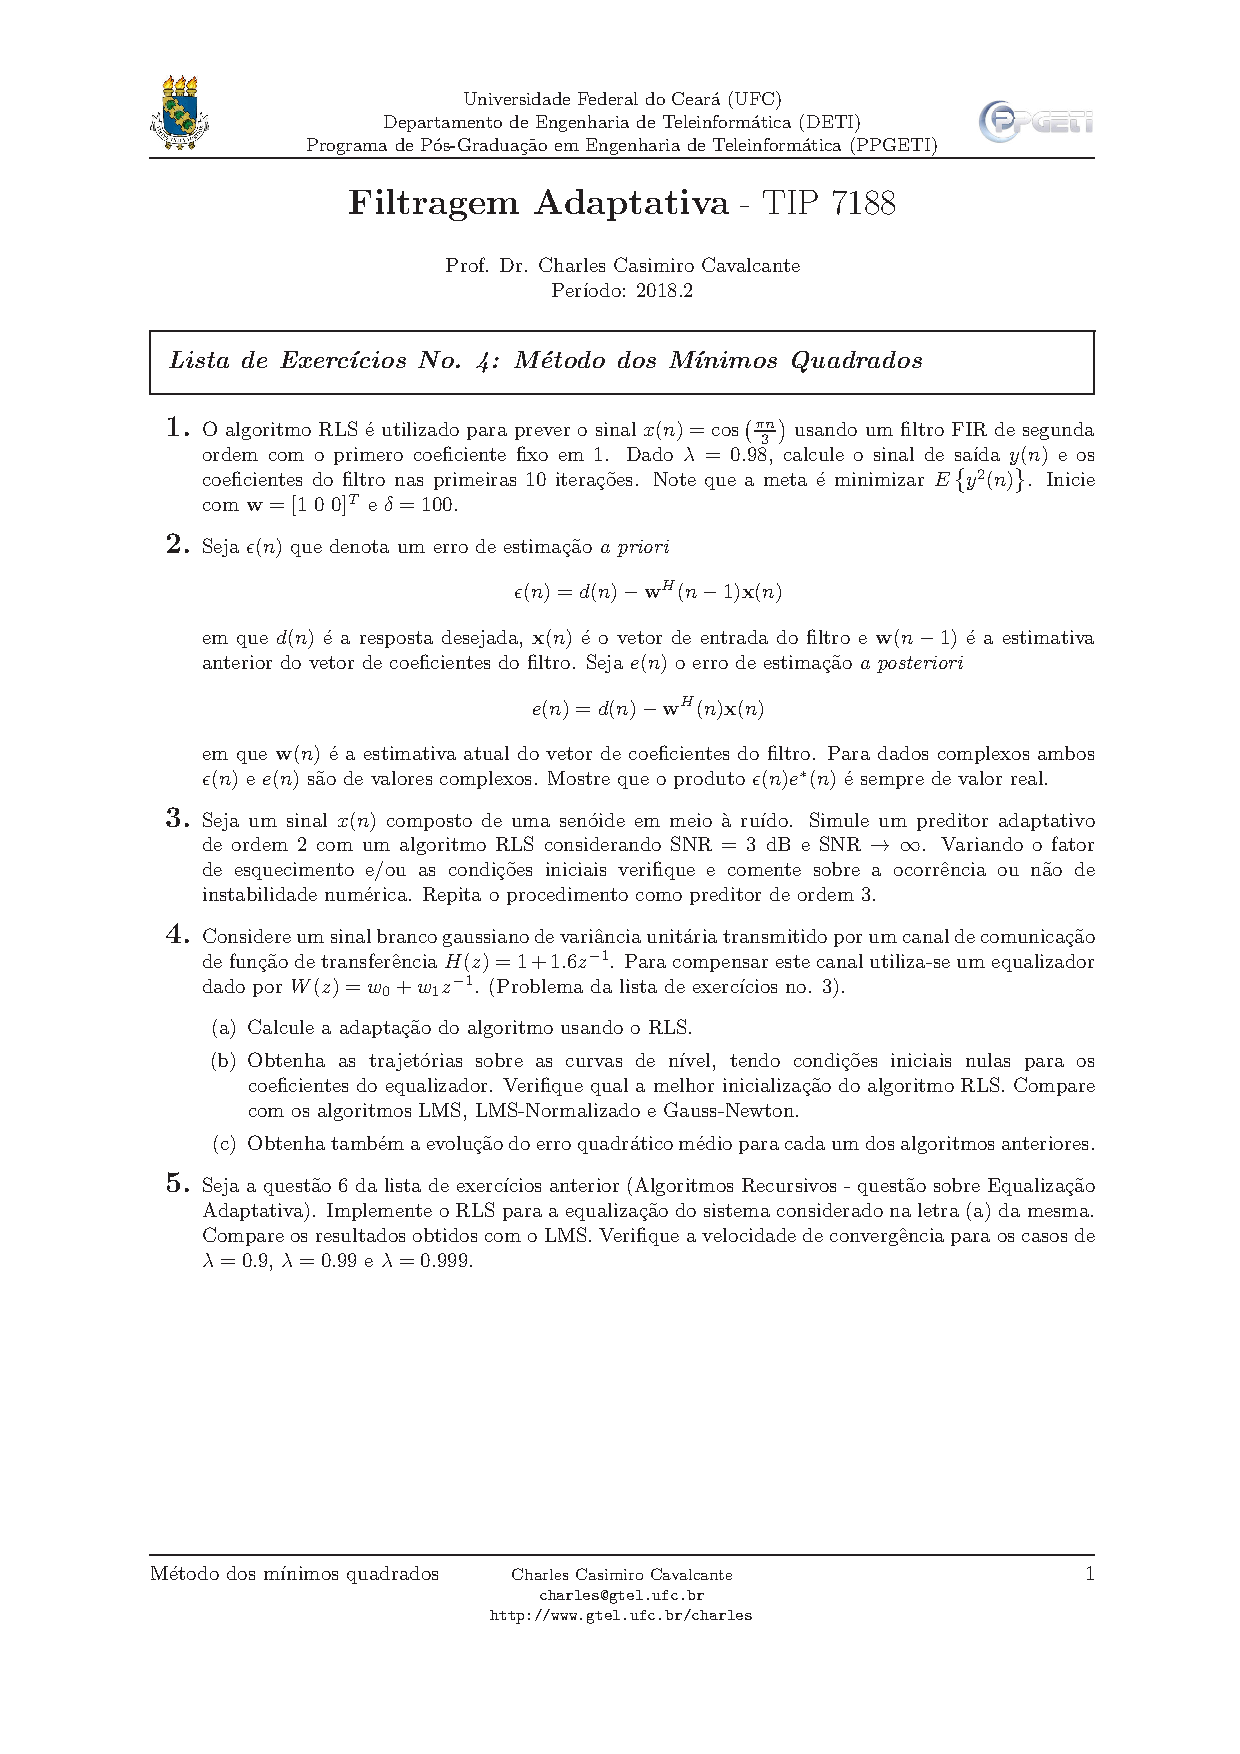
\includepdf[pages={-},addtotoc={1,subsection,1, Exercícios Propostos,p4}]{C:/Users/lucasabdalah-dell/Documents/GitHub/Courses-HWs/Master/TIP7188-FILTRAGEM_ADAPTATIVA/homework/report/listas/Lista_exercicios_4.pdf}
\clearpage

\section{Implementações em MATLAB}
A implementação é dividida em dois arquivos. O primeiro é chamado \textit{filter\_hw.m}\footnote{\textit{filter\_hw.m}: \url{https://github.com/lucasabdalah/Courses-HWs/blob/master/Master/TIP7188-FILTRAGEM_ADAPTATIVA/homework/code/filter_hw.m}}, onde há a definição dos métodos utilizados nos problemas. O segundo é o script \textit{main.m}\footnote{\textit{main.m}: \url{https://github.com/lucasabdalah/Courses-HWs/blob/master/Master/TIP7188-FILTRAGEM_ADAPTATIVA/homework/code/main.m}.}, que chama os métodos para serem executados. São apresentados nas sessões~\ref{p5} e \ref{p6}, respectivamente.




% \vspace*{\fill}   
% \centering
% \large \textit{Página Intencionalmente em Branco} % this page intentionally left blank
% \vspace*{\fill}

\clearpage
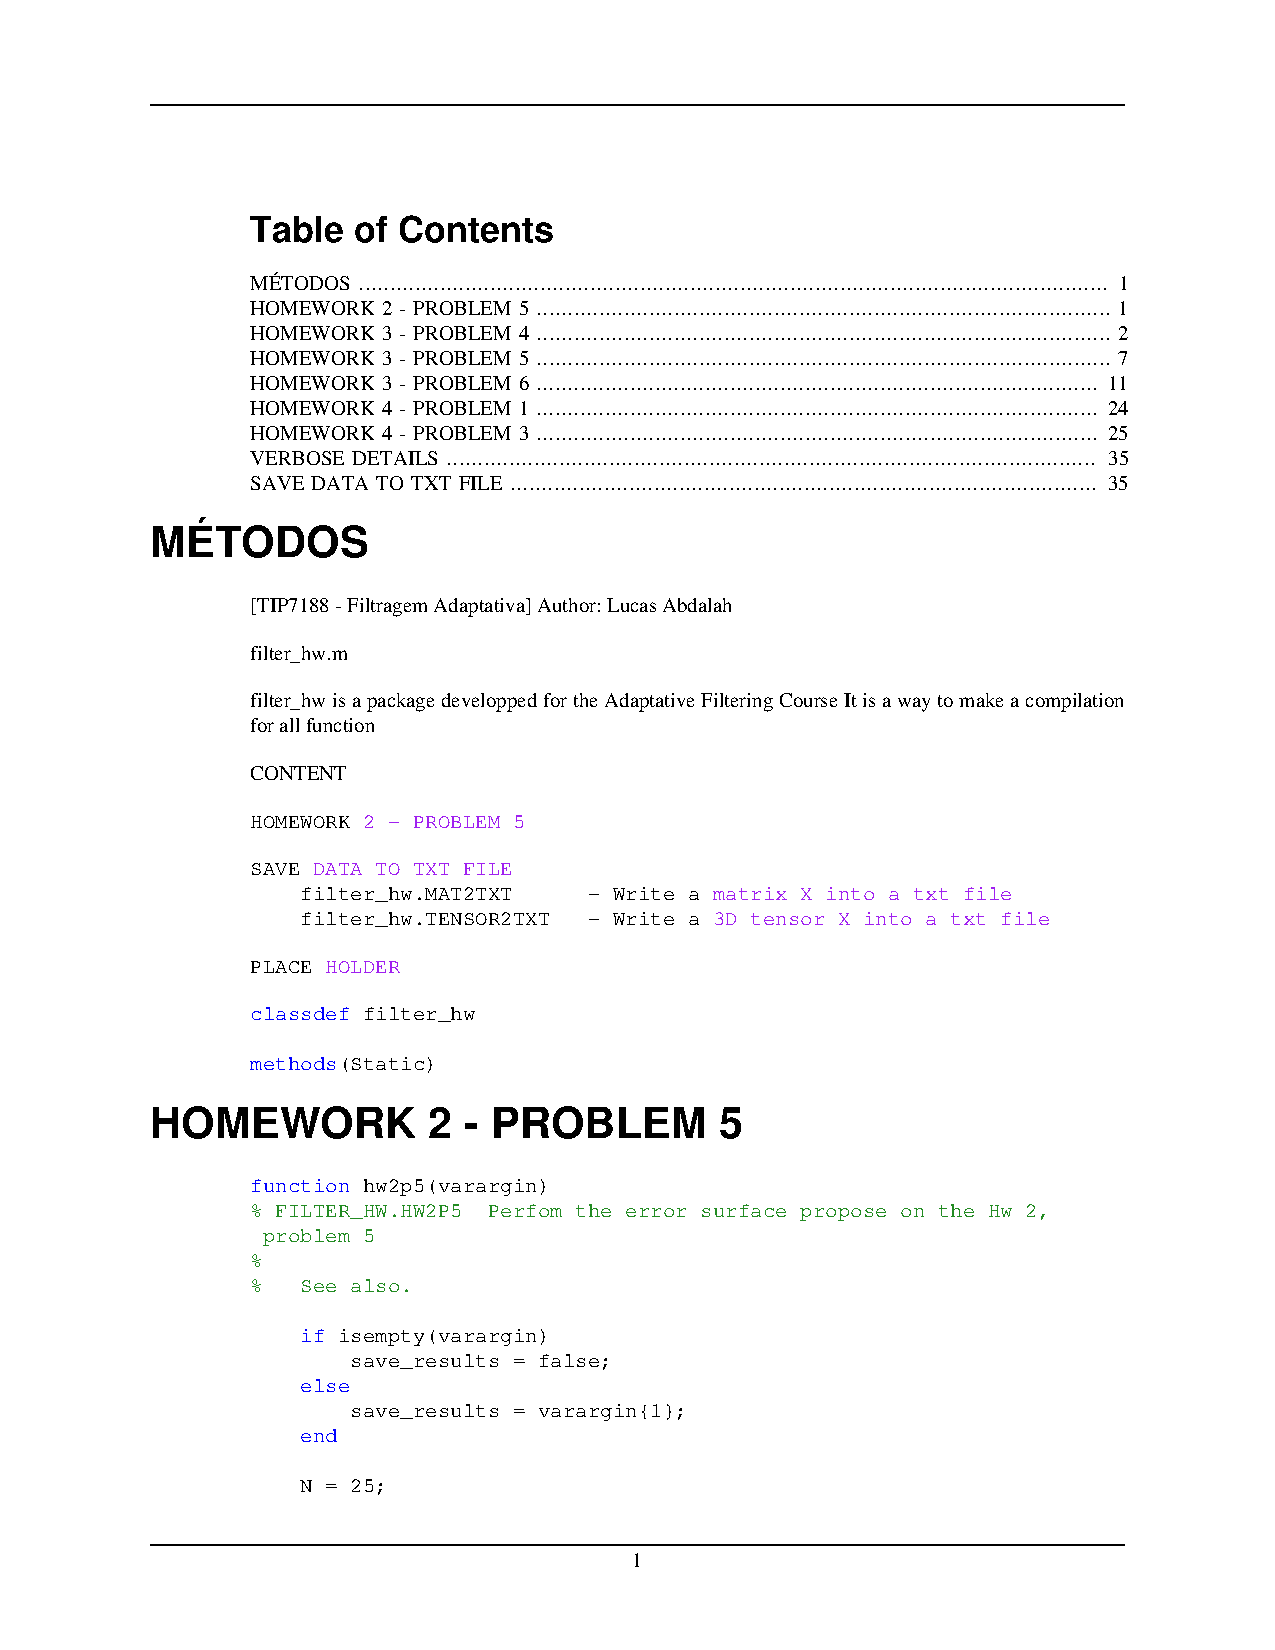
\includepdf[pages={-},addtotoc={1,subsection,1, Métodos, p5}]{C:/Users/lucasabdalah-dell/Documents/GitHub/Courses-HWs/Master/TIP7188-FILTRAGEM_ADAPTATIVA/homework/code/html/filter_hw.pdf}
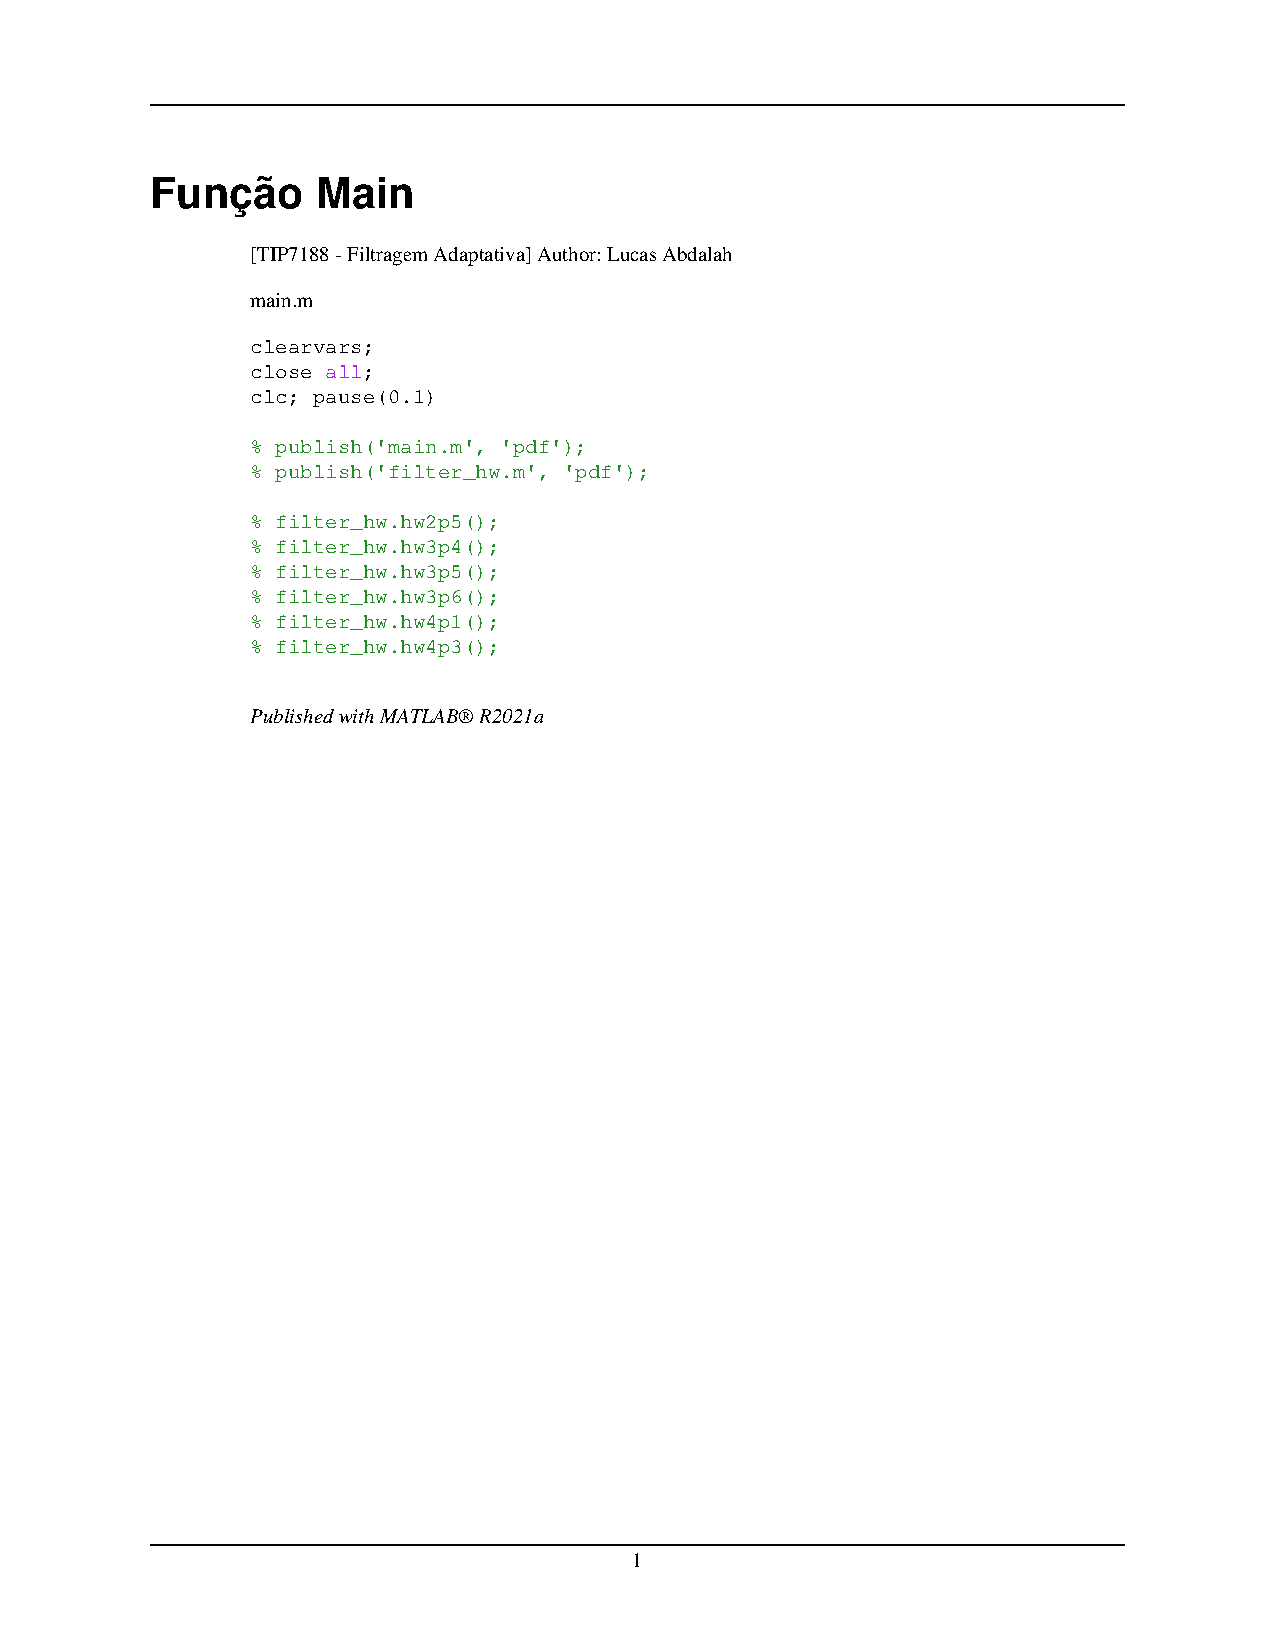
\includepdf[pages={-},addtotoc={1,subsection,1, Função Main, p6}]{C:/Users/lucasabdalah-dell/Documents/GitHub/Courses-HWs/Master/TIP7188-FILTRAGEM_ADAPTATIVA/homework/code/html/main.pdf}


% Bibliografia
% LateX vai gerar as ``Referências'' automaticamente
% usando a função \cite{nome} do pacote BibTeX é possível
% "puxar todas as informações do arquivo 'refs.bib'
% O nome do arquivo é o primeiro parâmetro de cada referência
% Um exemplo esta é utilizado na primeira seção
% \AtNextBibliography{\small}             % To set a smaller font size for bibliography
% \printbibliography[heading=bibintoc]    % Print the references

\end{document}